\documentclass[a4paper,12pt]{article}
\usepackage{polski}
\usepackage[utf8]{inputenc}
\usepackage[left = 3cm, right = 3cm, top = 2cm, bottom = 2cm]{geometry}
\usepackage{enumerate}
\usepackage{amssymb}		% pakiet do symboli
\usepackage{mathtools}		% pakiet do matmy (rozszerza amsmath)
\usepackage{enumitem}		% punktowanie (a), (b), ...
\usepackage{nopageno}		% brak numerow stron
\usepackage{graphicx}		% wstawianie obrazkow
\usepackage{float}			% wstawianie obrazkow w dowolnym miejscu
\usepackage{caption}
\usepackage{esdiff}         % pochodne \diff{}{}
\usepackage{listings}
\usepackage{xcolor}
\usepackage{adjustbox}
\usepackage{tkz-graph}
%\usepackage[none]{hyphenat} % usunięcie łamania wyrazów na końcu linii

% nowe komendy dla wygodniejszego pisania :)

\newcommand{\floor}[1]{\left\lfloor #1 \right\rfloor}	% podłoga
\newcommand{\ceil}[1]{\left\lceil #1 \right\rceil}		% sufit
\newcommand{\fractional}[1]{\left\{ #1 \right\}}		% część ułamkowa {x}
\newcommand{\abs}[1]{\left| #1 \right|}					% wartosc bezwzgledna / moc
\newcommand{\set}[1]{\left \{ #1 \right \}}				% zbiór elementów {a,b,c}
\newcommand{\pair}[1]{\left( #1 \right)}				% para elementów (a,b)
\newcommand{\Mod}[1]{\ \mathrm{mod\ #1}}				% lekko zmodyfikowane modulo
\newcommand{\comp}[1]{\overline{ #1 }} 					% dopełnienie zbioru 
\newcommand{\annihilator}{\mathbf{E}}					% operator E
\newcommand{\seqAnnihilator}[1]{\annihilator \left\langle #1 \right\rangle} % E(a_n)
\newcommand{\sequence}[1]{\left\langle #1 \right\rangle} % <a_n>
\DeclareMathOperator{\lcm}{lcm}							% obsługa lcm w mathmode

% styl do kodu
\lstdefinestyle{code}{%
basicstyle=\ttfamily\small,
commentstyle=\color{green!60!black},
keywordstyle=\color{magenta},
stringstyle=\color{blue!50!red},
showstringspaces=false,
numbers=left,
numberstyle=\footnotesize\color{gray},
numbersep=10pt,
tabsize=4,
rulecolor=\color{red},
breaklines=true
}

\newcommand{\code}[1]{\lstinline[style=code]{#1}} % kod inline

\begin{document}
\noindent \textbf{Sieci komputerowe, Ćwiczenia 1 - Tomasz Woszczyński}\newline

\noindent \newline \textbf{Zadanie 1} \newline
Dla każdego z podanych poniżej adresów IP w notacji CIDR określ, czy jest to
adres sieci, adres rozgłoszeniowy czy też adres komputera. W każdym przypadku
wyznacz odpowiadający mu adres sieci, rozgłoszeniowy i jakiś adres IP innego
komputera w tej samej sieci.

\begin{itemize}
    \item $10.1.2.3/8$
    \item $157.17.0.0/16$
    \item $99.99.99.99/27$
    \item $156.17.64.4/30$
    \item $123.123.123.123/32$
\end{itemize}

\noindent Dla maski $n$-bitowej adresem sieci jest adres mający pierwsze $n$ bitów
ustawionych, a pozostałe wyzerowane (bity odpowiadające za adres hosta). Adres
rozgłoszeniowy w części odpowiadającej za adres hosta ma same jedynki. \\

\noindent Przykład (1): Adres $10.1.2.3/8$ jest adresem komputera. Adresem 
sieci jest $10.0.0.0$, adresem rozgłoszeniowym $10.255.255.255$, a innym
adresem komputera w tej sieci $10.0.0.1$. \\

\noindent Przykład (2): Adres $157.17.0.0/16$ jest adresem sieci. Adresem
rozgłoszeniowym jest $157.17.0.0/16$, a jakimś adresem komputera w tej sieci
jest $157.17.0.1$. \\

\noindent Przykład (3): Adres $99.99.99.99/27$ jest adresem komputera. Adresem
sieci jest $99.99.99.96$, adresem rozgłoszeniowym $99.99.99.127$, a innym
adresem komputera w tej sieci $99.99.99.100$. \\

\noindent Przykład (4): Adres $156.17.64.4/30$ jest adresem sieci. Adresem 
rozgłoszeniowym jest $156.17.64.7$, a jakimś adresem komputera w tej sieci
jest $156.17.64.5$. \\

\noindent Przykład (5): Adres $123.123.123.123/32$ jest pojedynczym adresem
IP komputera. Prefiks jest $32$-bajtowy, a więc adres komputera jest 
jednocześnie adresem sieci oraz adresem rozgłoszeniowym.

\noindent \newline \textbf{Zadanie 2} \newline
Podziel sieć $10.10.0.0/16$ na $5$ rozłącznych podsieci, tak aby każdy z adresów
IP sieci $10.10.0.0/16$ był w jednej z tych $5$ podsieci. Jak zmieniła się liczba
adresów IP możliwych do użycia przy adresowaniu komputerów? Jaki jest minimalny
rozmiar podsieci, który możesz uzyskać w ten sposób? \\

\noindent Liczba adresów IP możliwych do użycia zmniejszy się. Spowodowane jest
to tym, że każda sieć ma przypisany jeden adres sieci oraz jeden adres 
rozgłoszeniowy. Skoro mieliśmy jedną sieć (2 adresy), a teraz mamy 5 sieci
(10 takich adresów), to stracimy 8 adresów IP, które moglibyśmy wykorzystać. \\

\noindent Aby stworzyć 5 podsieci, potrzebujemy $\ceil{\log_2{5}} = 3$ bity.
Niech pierwsza podsieć ma bity $000$, druga $001$, trzecia $010$, czwarta $011$,
a piąta $100$. Skoro maska ma $16$ bitów, to pierwsze $16$ bitów adresu IP
pozostanie niezmienione, a wcześniej wypisane bity dla podsieci będą stały zaraz
po adresie IP. Mamy więc adresy:

\begin{enumerate}
    \item $00001010.00001010.\underbrace{000}_{0}00000.00000000 = 10.10.0.0/19$,
    \item $00001010.00001010.\underbrace{001}_{32}00000.00000000 = 10.10.32.0/19$,
    \item $00001010.00001010.\underbrace{010}_{64}00000.00000000 = 10.10.64.0/19$,
    \item $00001010.00001010.\underbrace{011}_{96}00000.00000000 = 10.10.96.0/19$,
    \item $00001010.00001010.\underbrace{100}_{128}00000.00000000 = 10.10.128.0/17$.
\end{enumerate}

\noindent Maska 5. adresu jest mniejsza, jako że chcemy objąć wszystkie adresy
IP używane wcześniej, przed podziałem. Aby uzyskać najmniejszy rozmiar podsieci,
zacznijmy tworzenie sieci od tej, która zawiera najwięcej adresów IP, a następnie
dzielmy mniejsze sieci. Uzyskamy dzięki temu następujący podział:

\begin{enumerate}
    \item $10.10.128.0/17$,
    \item $10.10.64.0/18$,
    \item $10.10.32.0/19$,
    \item $10.10.16.0/20$,
    \item $10.10.0.0/20$.
\end{enumerate}

\noindent Minimalny rozmiar podsieci to $2^{32-20}-2 = 2^{12} - 2 = 4094$.

\newpage
\noindent \textbf{Zadanie 3} \newline
Tablica routingu zawiera następujące wpisy (podsieć $\to$ dokąd wysłać):
\begin{center}
\begin{tabular}{|l|c|l|l|}
    \hline
    Podsieć        & Dokąd wyłać  & Początek    & Koniec \\ 
    \hline
    0.0.0.0/0      & do routera A & 0.0.0.0     & 255.255.255.255 \\
    10.0.0.0/23    & do routera B & 10.0.0.0    & 10.0.1.255 \\
    10.0.2.0/24    & do routera B & 10.0.2.0    & 10.0.2.255 \\
    10.0.3.0/24    & do routera B & 10.0.3.0    & 10.0.3.255 \\
    10.0.1.0/24    & do routera C & 10.0.1.0    & 10.0.1.255 \\
    10.0.0.128/25  & do routera B & 10.0.0.128  & 10.0.0.255 \\
    10.0.1.8/29    & do routera B & 10.0.1.8    & 10.0.1.15 \\
    10.0.1.16/29   & do routera B & 10.0.1.16   & 10.0.1.23 \\
    10.0.1.24/29   & do routera B & 10.0.1.24   & 10.0.1.31 \\ \hline
\end{tabular}
\end{center}

\noindent Napisz równoważną tablicę routingu zawierającą jak najmniej wpisów. \\

\noindent Wpisy $10.0.2.0/24$ oraz $10.0.3.0/24$ możemy "skleić" w jeden wpis,
jako że zakresy tych podsieci są ze sobą "połączone", a więc z ostatniego adresu
pierwszej podsieci możemy przejść do pierwszego adresu drugiej podsieci. Oznacza
to, że te dwa wpisy stworzą jeden: $10.0.2.0/23$. Po takiej operacji możemy
"skleić" nowy wpis z wpisem $10.0.0.0/23$, tworząc zakres $10.0.0.0/22$. Wpis 
$10.0.0.128/25$ jest podzbiorem wpisu $10.0.0.0/22$, więc możemy go usunąć. \\

\noindent Podobną operację można wykonać dla dwóch ostatnich wpisów, czyli 
łączymy podsieci $10.0.1.16/29$ z $10.0.1.24/29$ i otrzymujemy $10.0.1.16/28$. \\

\noindent Po takich operacjach otrzymujemy nową, zmniejszoną tablicę routingu:
\begin{center}
    \begin{tabular}{|l|c|l|l|}
        \hline
        Podsieć        & Dokąd wyłać  & Początek    & Koniec \\ 
        \hline
        0.0.0.0/0      & do routera A & 0.0.0.0     & 255.255.255.255 \\
        10.0.0.0/22    & do routera B & 10.0.0.0    & 10.0.3.255 \\
        10.0.1.0/24    & do routera C & 10.0.1.0    & 10.0.1.255 \\
        10.0.1.8/29    & do routera B & 10.0.1.8    & 10.0.1.15 \\
        10.0.1.16/28   & do routera B & 10.0.1.16   & 10.0.1.31 \\ \hline
    \end{tabular}
\end{center}

\noindent \newline \textbf{Zadanie 4} \newline
Wykonaj powyższe zadanie dla tablicy
\begin{center}
    \begin{tabular}{|l|c|l|l|}
        \hline
        Podsieć        & Dokąd wyłać  & Początek    & Koniec \\ 
        \hline
        0.0.0.0/0      & do routera A & 0.0.0.0     & 255.255.255.255 \\
        10.0.0.0/8     & do routera B & 10.0.0.0    & 10.255.255.255 \\
        10.3.0.0/24    & do routera C & 10.3.0.0    & 10.3.0.255 \\
        10.3.0.32/27   & do routera B & 10.3.0.32   & 10.3.0.63 \\
        10.3.0.64/27   & do routera B & 10.3.0.64   & 10.3.0.95 \\
        10.3.0.96/27   & do routera B & 10.3.0.96   & 10.3.0.127 \\ \hline
    \end{tabular}
\end{center}

\noindent Wpisy $10.3.0.64/27$ i $10.3.0.96/27$ można skleić w jeden, dzięki
czemu powstanie wpis $10.3.0.64/26$. \\

\noindent Warto zauważyć, że router C obsługuje zakres adresów od $10.3.0.32$ 
do $10.3.0.127$, który jest obsługiwany przez router B. Oznacza to, że wpis
dla routera C można rozbić na dwa (na obrazku przedstawione czystym zielonym
kolorem, bez dodatku czerwonego), a wpisy routera B nad zielonym fragmentem
całkowicie usunąć (bo są obsługiwane przez wpis $10.0.0.0/8$). Wtedy powstałby
jeden nowy wpis, ale pozbylibyśmy się dwóch, więc tablica routingu byłaby
mniejsza.

\begin{figure}[H]
    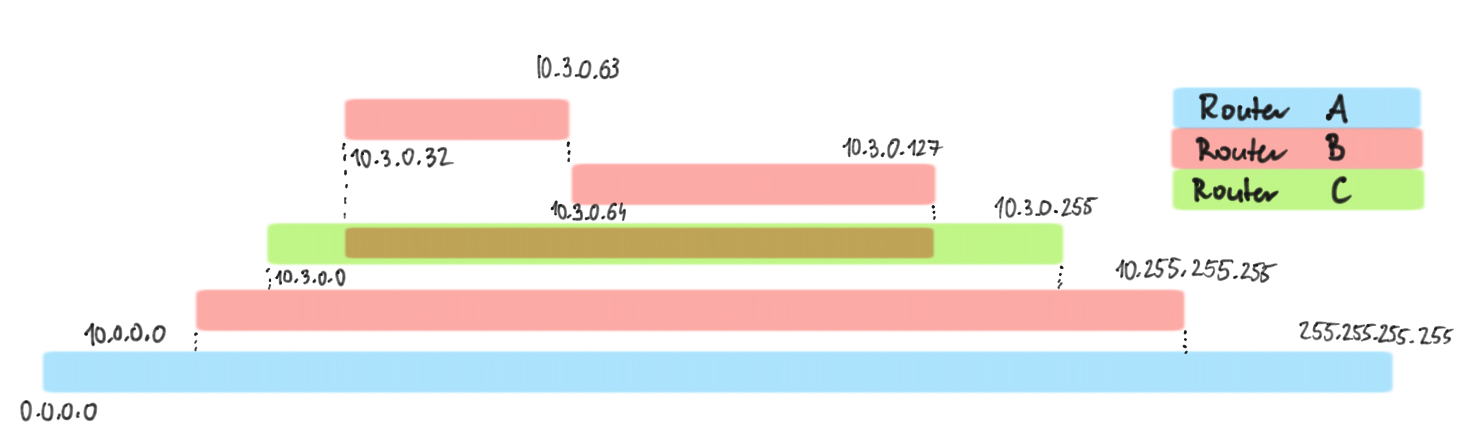
\includegraphics[width=\textwidth]{Pomocnicze/zadanie04.png}
\end{figure}

\noindent Po wykonaniu takich optymalizacji otrzymamy taką tablicę routingu:
\begin{center}
    \begin{tabular}{|l|c|l|l|}
        \hline
        Podsieć        & Dokąd wyłać  & Początek    & Koniec \\ 
        \hline
        0.0.0.0/0      & do routera A & 0.0.0.0     & 255.255.255.255 \\
        10.0.0.0/8     & do routera B & 10.0.0.0    & 10.255.255.255 \\
        10.3.0.0/27    & do routera C & 10.3.0.0    & 10.3.0.31 \\
        10.3.0.128/25  & do routera C & 10.3.0.128  & 10.3.0.255 \\ \hline
    \end{tabular}
\end{center}

\noindent \newline \textbf{Zadanie 5} \newline
Jak uporządkować wpisy w tablicy routingu, żeby zasada najlepszego dopasowania
odpowiadała wyborowi "pierwszy pasujący" (tj. przy przeglądaniu tablicy od
początku do końca aż do momentu napotkania dowolnej pasującej reguły)? Odpowiedź
uzasadnij formalnie. \\

\noindent Wpisy w tablicy routingu dopasowujemy po najdłuższym pasującym
prefiksie, a więc uporządkowujemy wpisy od najdłuższych pasujących prefiksów do
najkrótszych. Jeżeli jakieś wpisy mają taką samą długość prefiksu, to nie musimy
ich sortować. \\

\noindent \textbf{Dowód:} Załóżmy, że wpisy w tablicy routingu są uporządkowane
od najdłuższych pasujących prefiksów do najkrótszych. Udowodnimy, że wybór
pierwszego pasującego wpisu prowadzi do najlepszego dopasowania. \\

\noindent Weźmy dowolny adres IP, oznaczmy go jako $x$. Niech $y$ będzie 
pierwszym w kolejności rozpatrywania wpisem w tablicy routingu, do którego 
pasuje $x$. Przez $n$ oznaczmy długość prefiksu $y$, a skoro $x$ pasuje do $y$,
to pierwsze $n$ bitów $x$ oraz $y$ są identyczne. Weźmy teraz dowolny wpis $z$
będący w tablicy routingu za $y$. Oznacza to, że $z$ ma mniejszy prefiks od $y$,
a więc długość $m$ prefiksu $z$ spełnia nierówność $m \leq n$. Skoro tak, to
dopasowane zostanie nie więcej bitów $x$ niż $n$, czyli $y$ nie jest gorszym
dopasowaniem niż $z$, a więc wybór "pierwszy pasujący" odpowiada zasadzie
najlepszego dopasowania, co kończy dowód.

\newpage
\noindent \textbf{Zadanie 6} \newline
W podanej niżej sieci tablice routingu budowane są za pomocą algorytmu wektora
odległości. Pokaż (krok po kroku), jak będzie się to odbywać. W ilu krokach
zostanie osiągnięty stan stabilny?

\begin{figure}[H]
    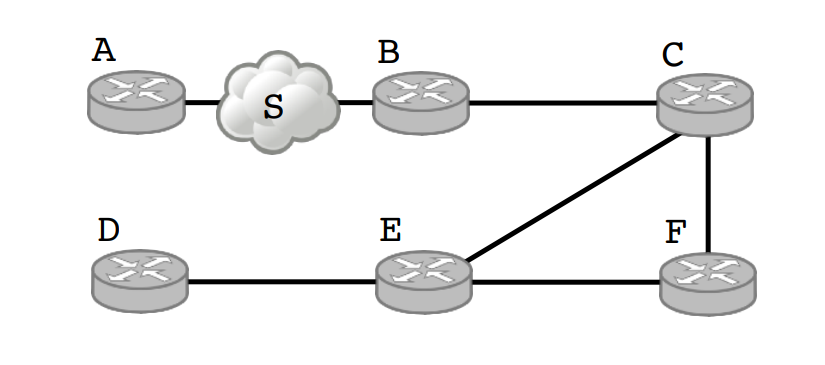
\includegraphics[width=\textwidth]{Pomocnicze/zadanie06.png}
\end{figure}

\noindent Algorytm wektora odległości polega na okresowym powiadamianiu sąsiadów
o całej swojej tablicy przekazywania. Oznacza to, że w każdym kroku tablica
routingu jest aktualizowana o nowe wpisy. Na początku oczywiście każdy zna tylko
swoich sąsiadów. W tabelce są to wpisy oznaczone przez "1", a puste komórki
oznaczają nieosiągalne (na ten moment) routery.

\begin{center}
    \begin{tabular}{|c|c|c|c|c|c|c|}
        \hline
        (krok 0.)   & A & B & C & D & E & F \\ \hline
        trasa do A  & - & 1 &   &   &   &   \\ \hline
        trasa do B  & 1 & - & 1 &   &   &   \\ \hline
        trasa do C  &   & 1 & - &   & 1 & 1 \\ \hline
        trasa do D  &   &   &   & - & 1 &   \\ \hline
        trasa do E  &   &   & 1 & 1 & - & 1 \\ \hline
        trasa do F  &   &   & 1 &   & 1 & - \\ \hline
        trasa do S  & 1 & 1 &   &   &   &   \\ \hline
    \end{tabular}
\end{center}

\begin{center}
    \begin{tabular}{|c|c|c|c|c|c|c|}
        \hline
        (krok 1.)   & A         & B         & C         & D         & E         & F         \\ \hline
        trasa do A  & -         & 1         & 2 (via B) &           &           &           \\ \hline
        trasa do B  & 1         & -         & 1         &           & 2 (via C) & 2 (via C) \\ \hline
        trasa do C  & 2 (via B) & 1         & -         & 2 (via E) & 1         & 1         \\ \hline
        trasa do D  &           &           & 2 (via E) & -         & 1         & 2 (via D) \\ \hline
        trasa do E  &           & 2 (via C) & 1         & 1         & -         & 1         \\ \hline
        trasa do F  &           & 2 (via C) & 1         & 2 (via E) & 1         & -         \\ \hline
        trasa do S  & 1         & 1         & 2 (via B) &           &           &           \\ \hline
    \end{tabular}
\end{center}

\begin{center}
    \begin{tabular}{|c|c|c|c|c|c|c|}
        \hline
        (krok 2.)   & A         & B         & C         & D         & E         & F         \\ \hline
        trasa do A  & -         & 1         & 2 (via B) &           & 3 (via C) & 3 (via C) \\ \hline
        trasa do B  & 1         & -         & 1         & 3 (via E) & 2 (via C) & 2 (via C) \\ \hline
        trasa do C  & 2 (via B) & 1         & -         & 2 (via E) & 1         & 1         \\ \hline
        trasa do D  &           & 3 (via C) & 2 (via E) & -         & 1         & 2 (via E) \\ \hline
        trasa do E  & 3 (via B) & 2 (via C) & 1         & 1         & -         & 1         \\ \hline
        trasa do F  & 3 (via B) & 2 (via C) & 1         & 2 (via E) & 1         & -         \\ \hline
        trasa do S  & 1         & 1         & 2 (via B) &           & 3 (via C) & 3 (via C) \\ \hline
    \end{tabular}
\end{center}

\begin{center}
    \begin{tabular}{|c|c|c|c|c|c|c|}
        \hline
        (krok 3.)   & A         & B         & C         & D         & E         & F         \\ \hline
        trasa do A  & -         & 1         & 2 (via B) & 4 (via E) & 3 (via C) & 3 (via C) \\ \hline
        trasa do B  & 1         & -         & 1         & 3 (via E) & 2 (via C) & 2 (via C) \\ \hline
        trasa do C  & 2 (via B) & 1         & -         & 2 (via E) & 1         & 1         \\ \hline
        trasa do D  & 4 (via B) & 3 (via C) & 2 (via E) & -         & 1         & 2 (via E) \\ \hline
        trasa do E  & 3 (via B) & 2 (via C) & 1         & 1         & -         & 1         \\ \hline
        trasa do F  & 3 (via B) & 2 (via C) & 1         & 2 (via E) & 1         & -         \\ \hline
        trasa do S  & 1         & 1         & 2 (via B) & 4 (via E) & 3 (via C) & 3 (via C) \\ \hline
    \end{tabular}
\end{center}

\noindent Po wykonaniu tych trzech kroków został osiągnięty stan stabilny, a więc
wszystkie routery w sieci znają już drogę do wszystkich pozostałych routerów 
i wyznaczone ścieżki są najkrótszymi ścieżkami.

\noindent \newline \textbf{Zadanie 7} \newline
Załóżmy, że w powyższej sieci tablice routingu zostały już zbudowane. Co będzie
się działo, jeśli zostanie dodane połączenie między routerami A i D? \\

\noindent Po dodaniu połączenia między A i D otrzymamy taką sieć:
\begin{figure}[H]
    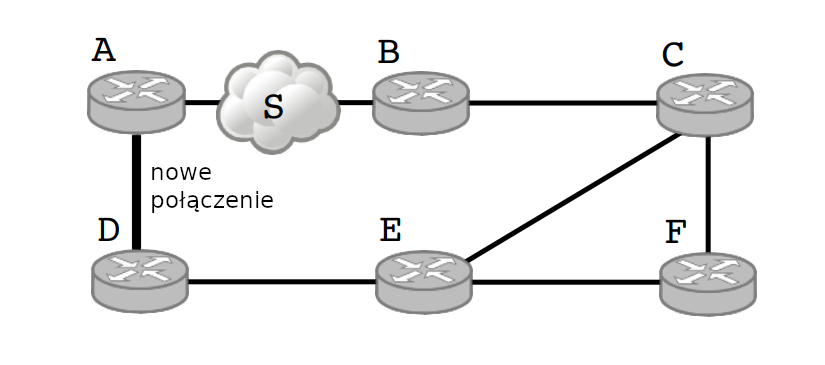
\includegraphics[width=\textwidth]{Pomocnicze/zadanie07.png}
\end{figure}

\noindent W zerowym kroku mamy taką tablicę jaką otrzymaliśmy na koniec zadania 6, 
jednak teraz routery A i D muszą się o sobie dowiedzieć. Z tego powodu początkowa 
tablica routingu wygląda tak:

\begin{center}
    \begin{tabular}{|c|c|c|c|c|c|c|}
        \hline
        (krok 0.)   & A         & B         & C         & D         & E         & F         \\ \hline
        trasa do A  & -         & 1         & 2 (via B) & 1         & 3 (via C) & 3 (via C) \\ \hline
        trasa do B  & 1         & -         & 1         & 3 (via E) & 2 (via C) & 2 (via C) \\ \hline
        trasa do C  & 2 (via B) & 1         & -         & 2 (via E) & 1         & 1         \\ \hline
        trasa do D  & 1         & 3 (via C) & 2 (via E) & -         & 1         & 2 (via E) \\ \hline
        trasa do E  & 3 (via B) & 2 (via C) & 1         & 1         & -         & 1         \\ \hline
        trasa do F  & 3 (via B) & 2 (via C) & 1         & 2 (via E) & 1         & -         \\ \hline
        trasa do S  & 1         & 1         & 2 (via B) & 4 (via E) & 3 (via C) & 3 (via C) \\ \hline
    \end{tabular}
\end{center}

\noindent Wiedząc, że powstała nowa ścieżka między routerami A i D, inne mogą
ulec skróceniu, w trakcie wymieniania się swoimi tablicami routingu.

\begin{center}
    \begin{tabular}{|c|c|c|c|c|c|c|}
        \hline
        (krok 1.)   & A         & B         & C         & D         & E         & F         \\ \hline
        trasa do A  & -         & 1         & 2 (via B) & 1         & 2 (via D) & 3 (via C) \\ \hline
        trasa do B  & 1         & -         & 1         & 2 (via A) & 2 (via C) & 2 (via C) \\ \hline
        trasa do C  & 2 (via B) & 1         & -         & 2 (via E) & 1         & 1         \\ \hline
        trasa do D  & 1         & 2 (via A) & 2 (via E) & -         & 1         & 2 (via E) \\ \hline
        trasa do E  & 2 (via D) & 2 (via C) & 1         & 1         & -         & 1         \\ \hline
        trasa do F  & 3 (via B) & 2 (via C) & 1         & 2 (via E) & 1         & -         \\ \hline
        trasa do S  & 1         & 1         & 2 (via B) & 2 (via A) & 3 (via C) & 3 (via C) \\ \hline
    \end{tabular}
\end{center}

\noindent Po jednym kroku zostaje osiągnięty stan stabilny i wszystkie ścieżki
w tablicy routingu są już najkrótsze.

\end{document}